Before entering in the detail of the RACECAR model description we want to give a small introduction about the Gazebo 
simulator environment and the URDF/SDF description standard.

\section{Gazebo Simulator}
Gazebo is an open-source 3D dynamic simulator with the ability to accurately and efficiently simulate populations
of robots in complex indoor and outdoor environments. \\ 
It integrates the ODE physics engine to provide a high fidelity physics simulation, OpenGL rendering to have visually
appealing scenarios, and it supports code for sensor simulation and actuator control

\subsection{ODE}
The ODE (\textit{Open Dynamics Engine}) is a physics engine for simulating articulated rigid body dynamics.
It is fast, flexible, robust and has built-in collision detection.\\
An articulated structure is created when rigid bodies of various shapes are connected together with joints of various kinds.\\
ODE is designed to be used in interactive and real-time simulations. It has hard contacts, this means that a special 
non-penetration constraint is used whenever two bodies collide. \\
ODE uses the notion of \textit{Coulomb Friction}, which is the most common friction model. \\
The simplified friction law is: 
\[
F_c = \begin{cases} 
        \mu N \cdot sign(v) & \text{if $|v|>0$} \\
        \min(|F_{app}|,\ \mu N) \cdot sign(F_{app}) & \text{if $v=0$}
      \end{cases}
\] \\

\begin{figure}[H]
    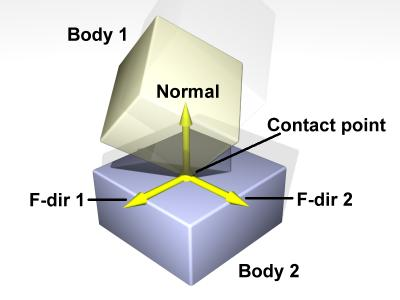
\includegraphics[scale = 0.7, width=\textwidth]{contact.jpg}
    \caption{Body interaction causing friction}
\end{figure}

Where $F_c$ is the Coulomb friction force, $v$ is the sliding speed, $\mu$ is the coefficient of friction, $N$ is the 
normal contact force and $F_{app}$ is the applied force on the body. \\

\section{URDF and SDF}
URDF (\textit{Unified Robot Description Format}) is an XML format for representing a robot model used by ROS. \\
A number of different packages and components compose URDF: \\

\begin{figure}[H]
    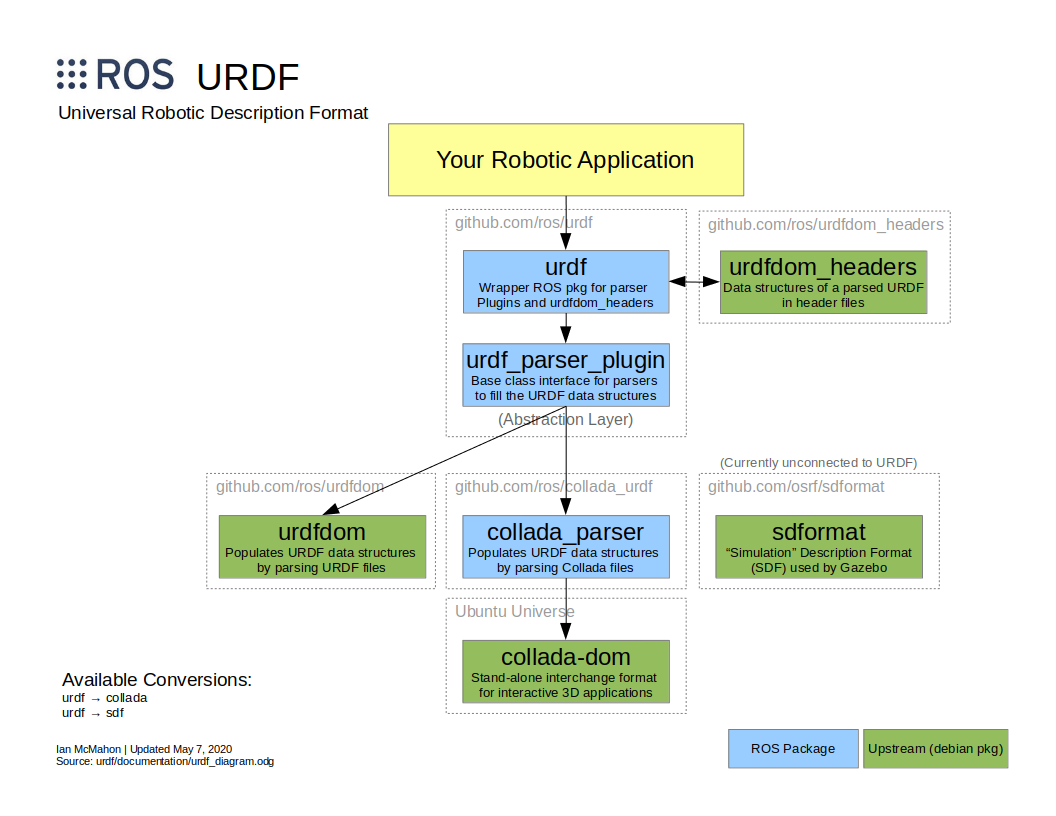
\includegraphics[width=\textwidth]{urdf_diagram.png}
    \caption{URDF description}
\end{figure}

URDF can only specify the kinematic and dynamic properties of a single robot in isolation, it cannot specify the pose 
of the robot itself with respect to the world it is placed in.\\
URDF is not a universal description format since it cannot specify joint loops (parallel linkages), and it lacks the possibility 
of specifying friction and other dynamic properties.\\
For the reasons above, Gazebo uses another XML format called SDF (\textit{Simulation Description Format}) which 
is a complete description for everything from the world level down to the robot level.\\ 
It has been developed also a macro language called XACRO (\textit{XML Macro}) to make it easier to maintain the robot description 
files, increase their readability, and to avoid duplication of code in the robot description files.
In our case, the model is described using XACRO files, and then it is converted to SDF by the \textit{gazebo\_ros} package.
Finally, it is spawned it in the Gazebo simulated world. \\
The basic building blocks for describing a robot using URDF/SDF are \textit{links} and \textit{joints}.

\subsection{Links}
In URDF/SDF, a \textit{Link}\footnote{Visit \url{https://wiki.ros.org/urdf/XML/link} for a detailed description} 
element describes a rigid body with an inertia, visual features, and collision properties. \\

\begin{figure}[H]
    \centering
    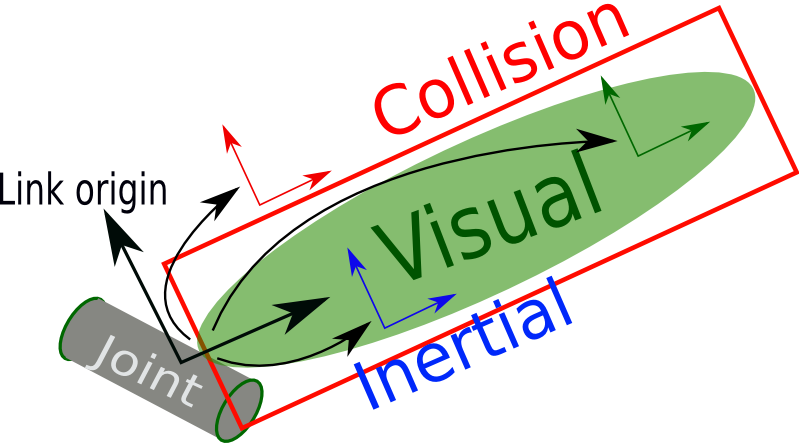
\includegraphics[scale=2]{inertial.png}
    \caption{Link schematic}
\end{figure}

Each \textit{link} element is composed by three main parts (encapsulated in their respective XML tags): 
\begin{itemize}
    \item \textit{Inertial} in which we specify the link mass, position of its center of mass, and its central inertia properties;
    \item \textit{Visual} in which we describe the shape of the object (e.g. box, cylinder) for visualization purposes. 
            We can also use multiple instances of <visual> tags for the same link to define the shape in a constructive way.
    \item \textit{Collision} in which we list the collision properties of a link, which are usually different from the visual ones. 
            In fact, simpler collision models are often used to reduce computation time. \\
            Also in this case, we can also use multiple instances of <collision> tags for the same link to define
            the desired shape in a constructive way.     
\end{itemize}


\subsection{Joints}
The \textit{joint}\footnote{Visit \url{https://wiki.ros.org/urdf/XML/joint} for a detailed description} 
element describes the kinematics, dynamics and safety limits of a joint connecting together two link objects.\\

\begin{figure}[H]
    \centering
    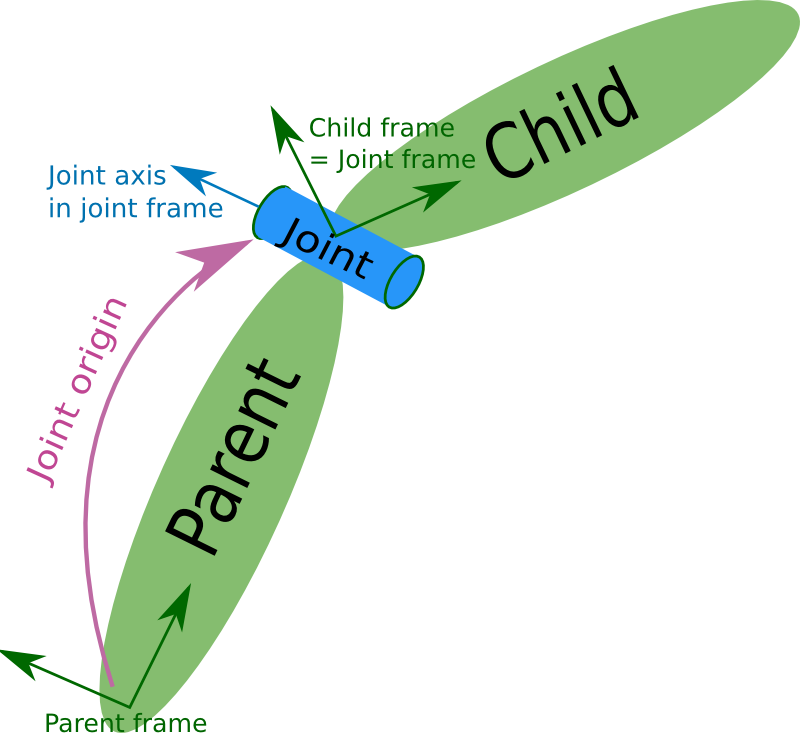
\includegraphics[scale=0.3]{joint.png}
    \caption{Joint schematic}
\end{figure}

Using the attribute \textit{type} we can specify the type of the joint as one of the following:
\begin{itemize}
    \item \textbf{revolute} — a hinge joint that rotates along the provided axis and has a limited range
                             specified by the upper and lower limits;
    \item \textbf{continuous} — a continuous hinge joint that rotates around the provided axis and has no upper and lower limits;
    \item \textbf{prismatic} — a sliding joint that slides along the axis, and has a limited range 
                                specified by the upper and lower limits;
    \item \textbf{fixed} — this is not really a joint because it cannot move since all degrees of freedom are locked. 
                            This type of joint is used to rigidly attach links together;
    \item \textbf{floating} — this joint allows motion for all 6 degrees of freedom;
    \item \textbf{planar} — this joint allows motion in a plane perpendicular to provided the axis. 
\end{itemize} 
Using <parent> and <child> XML elements, we can define which links (rigid bodies) are attached together through the joint. 

\subsection{URDF in Gazebo}
In order to use a robot described using URDF within Gazebo, it is mandatory that all links have an \textit{<inertial>} element. \\
Optionally, we can introduce additional information appending \textit{<gazebo>} elements to the links (e.g., to add sensor plugins
to convert colors to Gazebo format, ...), or to the joints (e.g., to set proper damping dynamics, add actuator control plugins, 
...).\footnote{Refer to \url{http://classic.gazebosim.org/tutorials?tut=ros_urdf} for a detailed guide on the conversion}


\section{RACECAR model description}
In this section we are going to explain the structure of the \textit{RACECAR project} developed by MIT, by focusing on 
the model the robot and on its simulation made by using Gazebo. \\
The robot is composed by nine links: a chassis, four wheels, two steering hinges, one Hokuyo LIDAR sensor and one camera;
and by eight joints: four for the wheels, two for the steering mechanism, and two for connecting the camera and the 
LIDAR to the car.\\

% racecar schematic
\begin{figure}[H]
    \makebox[\textwidth][c]{
    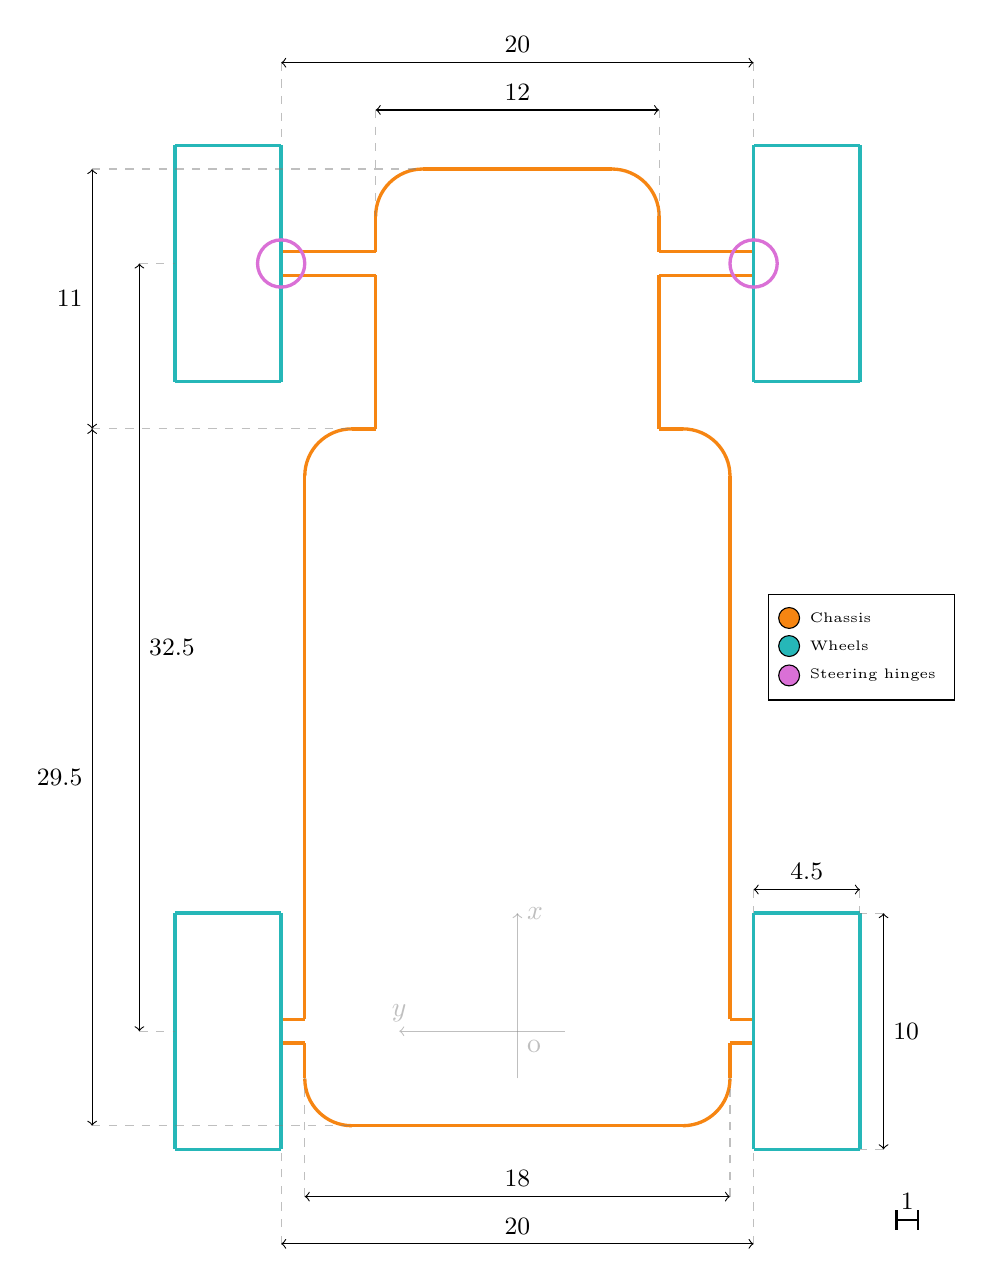
\begin{tikzpicture}[x=0.3cm,y=0.3cm] %set unit size along axes
        % axes (following Gazebo reference system)
        \draw[gray, opacity = 0.5,->] (0,-2) -- (0,5) node[right] {$x$};
		\draw[gray, opacity = 0.5,->] (2,0) -- (-5,0) node[above] {$y$};
		\draw[gray, opacity = 0.5] (0,0) node[below right] {o};

        %%% chassis %%%
        % rear left part
        \draw[very thick, BurntOrange] (-7,-4) -- (7,-4);
        \draw[very thick, BurntOrange] (-9,-2) -- (-9,-0.5);
        \draw[very thick, BurntOrange] (-9,-2) to[out=-90,in=180] (-7,-4); %rear left corner
        %rear left wheel axis
        \draw[very thick, BurntOrange] (-9,-0.5) -- (-10,-0.5);
        \draw[very thick, BurntOrange] (-10,-0.5) -- (-10,0.5);
        \draw[very thick, BurntOrange] (-10,0.5) -- (-9,0.5);
        %left part
        \draw[very thick, BurntOrange] (-9,0.5) -- (-9,23.5);
        \draw[very thick, BurntOrange] (-9,23.5) to[out=90,in=180] (-7,+25.5); %middle left corner
        \draw[very thick, BurntOrange] (-7,25.5) -- (-6,25.5);
        \draw[very thick, BurntOrange] (-6,25.5) -- (-6,32);
        %front left wheel axis
        \draw[very thick, BurntOrange] (-6,32) -- (-10,32);
        \draw[very thick, BurntOrange] (-10,32) -- (-10,33);
        \draw[very thick, BurntOrange] (-10,33) -- (-6,33);
        %front side
        \draw[very thick, BurntOrange] (-6,33) -- (-6,34.5);
        \draw[very thick, BurntOrange] (-6,34.5) to[out=90,in=180] (-4,36.5); %top left corner
        \draw[very thick, BurntOrange] (-4,36.5) -- (4,36.5);
        \draw[very thick, BurntOrange] (4,36.5) to[out=0,in=90] (6,34.5); %top right corner
        \draw[very thick, BurntOrange] (6,34.5) -- (6,33);
        %front right wheel axis
        \draw[very thick, BurntOrange] (6,32) -- (10,32);
        \draw[very thick, BurntOrange] (10,32) -- (10,33);
        \draw[very thick, BurntOrange] (10,33) -- (6,33);
        %right part
        \draw[very thick, BurntOrange] (9,0.5) -- (9,23.5);
        \draw[very thick, BurntOrange] (9,23.5) to[out=90,in=0] (7,+25.5); %middle left corner
        \draw[very thick, BurntOrange] (7,25.5) -- (6,25.5);
        \draw[very thick, BurntOrange] (6,25.5) -- (6,32);
        %rear right wheel axis
        \draw[very thick, BurntOrange] (9,-0.5) -- (10,-0.5);
        \draw[very thick, BurntOrange] (10,-0.5) -- (10,0.5);
        \draw[very thick, BurntOrange] (10,0.5) -- (9,0.5);
        % rear right part
        \draw[very thick, BurntOrange] (9,-2) -- (9,-0.5);
        \draw[very thick, BurntOrange] (9,-2) to[out=-90,in=0] (7,-4); %rear left corner

        %%% wheels %%%
        %rear left wheel%
        \draw[very thick, BlueGreen] (-10,-5) -- (-10,5);
        \draw[very thick, BlueGreen] (-10,-5) -- (-14.5,-5);
        \draw[very thick, BlueGreen] (-14.5,-5) -- (-14.5,5);
        \draw[very thick, BlueGreen] (-14.5,5) -- (-10,5);
        %top left wheel%
        \draw[very thick, BlueGreen] (-10,27.5) -- (-10,37.5);
        \draw[very thick, BlueGreen] (-10,27.5) -- (-14.5,27.5);
        \draw[very thick, BlueGreen] (-14.5,27.5) -- (-14.5,37.5);
        \draw[very thick, BlueGreen] (-14.5,37.5) -- (-10,37.5);
        %rear right wheel%
        \draw[very thick, BlueGreen] (10,-5) -- (10,5);
        \draw[very thick, BlueGreen] (10,-5) -- (14.5,-5);
        \draw[very thick, BlueGreen] (14.5,-5) -- (14.5,5);
        \draw[very thick, BlueGreen] (14.5,5) -- (10,5);
        %top right wheel%
        \draw[very thick, BlueGreen] (10,27.5) -- (10,37.5);
        \draw[very thick, BlueGreen] (10,27.5) -- (14.5,27.5);
        \draw[very thick, BlueGreen] (14.5,27.5) -- (14.5,37.5);
        \draw[very thick, BlueGreen] (14.5,37.5) -- (10,37.5);

        %steering hinges (circles of radius 1)
        \draw[very thick, Orchid] (-10, 32.5) circle[radius=1];
        \draw[very thick, Orchid] (10, 32.5) circle[radius=1];

        %%% legend %%%
	    \matrix [draw] at (current bounding box.east) {
        \node [circle, scale = 0.8, draw, fill= BurntOrange,label=right:\tiny Chassis] () {}; \\
        \node [circle, scale = 0.8, draw, fill= BlueGreen,label=right:\tiny Wheels] () {}; \\
        \node [circle, scale = 0.8, draw, fill= Orchid,label=right:\tiny Steering hinges] () {}; \\
        };
        
        \draw[thick, {Bar}-{Bar}] (16,-8) -- (17,-8) node[midway, above]{\small \SI{1}{\cm}};

        %%% measures %%%
        %back
        \draw[<->] (-9,-7) -- (9,-7) node[midway, above]{\small \SI{18}{\cm}};
        \draw[dashed, gray, opacity=0.5] (-9,-7) -- (-9,-2);
        \draw[dashed, gray, opacity=0.5] (9,-7) -- (9,-2);

        \draw[<->] (-10,-9) -- (10,-9) node[midway, above]{\small \SI{20}{\cm}};
        \draw[dashed, gray, opacity=0.5] (-10,-9) -- (-10,-5);
        \draw[dashed, gray, opacity=0.5] (10,-9) -- (10,-5);

        %wheel
        \draw[<->] (10,6) -- (14.5,6) node[midway, above]{\small \SI{4.5}{\cm}};
        \draw[dashed, gray, opacity=0.5] (10,6) -- (10,5);
        \draw[dashed, gray, opacity=0.5] (14.5,6) -- (14.5,5);

        \draw[<->] (15.5, -5) -- (15.5, 5) node[midway, right]{\small \SI{10}{\cm}};
        \draw[dashed, gray, opacity=0.5] (15.5, -5) -- (14.5,-5);
        \draw[dashed, gray, opacity=0.5] (15.5, 5) -- (14.5,5);

        %front
        \draw[<->] (-6,39) -- (6,39) node[midway, above]{\small \SI{12}{\cm}};
        \draw[dashed, gray, opacity=0.5] (-6, 39) -- (-6, 34.5);
        \draw[dashed, gray, opacity=0.5] (6, 39) -- (6, 34.5);

        \draw[<->] (-10,41) -- (10,41) node[midway, above]{\small \SI{20}{\cm}};
        \draw[dashed, gray, opacity=0.5] (-10, 41) -- (-10, 37.5);
        \draw[dashed, gray, opacity=0.5] (10, 41) -- (10, 37.5);

        %side
        \draw[<->] (-16, 0) -- (-16, 32.5) node[midway, right]{\small \SI{32.5}{\cm}};
        \draw[dashed, gray, opacity=0.5] (-16, 0) -- (-14.5, 0);
        \draw[dashed, gray, opacity=0.5] (-16, 32.5) -- (-14.5, 32.5);

        \draw[<->] (-18, -4) -- (-18, 25.5) node[midway, left]{\small \SI{29.5}{\cm}};
        \draw[dashed, gray, opacity=0.5] (-18, -4) -- (-7, -4);
        \draw[dashed, gray, opacity=0.5] (-18, 25.5) -- (-7, 25.5);
        \draw[<->] (-18, 25.5) -- (-18, 36.5) node[midway, left]{\small \SI{11}{\cm}};
        \draw[dashed, gray, opacity=0.5] (-18, 36.5) -- (-4, 36.5);


    \end{tikzpicture}}
    \caption{RACECAR links schematic}
    \label{fig:racecar}
\end{figure}

\subsection{RACECAR links}
\subsubsection{Chassis}
The robot chassis weights \SI{4}{\kilogram} and has an irregular shape (see schematic in \ref{fig:racecar}); 
it is placed \SI{5}{\cm} above the ground (\SI{0.05}{\metre} offset on the $z$ axis). Since there is 
no <collision> element, all collisions with the chassis are ignored.\\ 
The inertial matrix is: 
$$
\begin{bmatrix}
0.010609 & 0 & 0 \\
0 & 0.050409 & 0 \\
0 & 0 & 0.05865 \\
\end{bmatrix}
\quad
$$
It is a frictionless surface ($\mu_{1} = \mu_{2} = 0$), but has spring constant equals to \SI[per-mode = symbol]{1e7}{\newton\per\metre}
and a damping constant of \SI[per-mode = symbol]{1.0}{\kilogram\per\second}.

\subsubsection{Wheels}
Each one of the four wheels, weighting \SI{0.34}{\kilogram}, has a cylindrical shape with rounded borders defined 
by a custom STL (\textit{STereo Lithography interface format}) file. \\
The inertial matrix is reported here: 
$$
\begin{bmatrix}
0.00026046 & 0 & 0 \\
0 & 0.00026046 & 0 \\
0 & 0 & 0.00041226 \\
\end{bmatrix}
\quad
$$
Each wheel has also two friction coefficients, $\mu_{1}$ and $\mu_{2}$, both set to $1$; these coefficients 
are referring to the principal contact directions along the contact surface.
Furthermore, we have a spring constant of \SI[per-mode = symbol]{1e7}{\newton\per\metre} and a 
damping constant of \SI[per-mode = symbol]{1.0}{\kilogram\per\second}. \\
Since we are interested in the ground tire interaction, it is necessary to specify the first friction direction 
in the local reference frame along which frictional force is applied. Such vector must be of unit length and perpendicular 
to the contact normal, it is typically tangential to the contact surface: rear wheels have a friction direction 
vector equal to 
$\left[\begin{smallmatrix} 1 & 0 & 0 \end{smallmatrix}\right]$, instead front wheels have a friction 
direction vector equal to $\left[\begin{smallmatrix} 0 & 0 & 1 \end{smallmatrix}\right]$. \\
Each wheel has its own collision space, it is delimited by a cylinder \SI{4.5}{\cm} long and having a 
radius of \SI{5}{\cm}. The origin of the collision spaces for right wheels are shifted by
 $\left[\begin{smallmatrix} 0 & 0 & 0.0225 \end{smallmatrix}\right]$,
instead the origin of the collision spaces for the left wheels are shifted by
 $\left[\begin{smallmatrix} 0 & 0 & -0.0225 \end{smallmatrix}\right]$.
These translations, performed with respect to the joints frames (connecting the wheels to the chassis), are necessary
to align the generated collision cylinders with the visual geometries.
\footnote{At a first glance, different translations of the wheels along the $z$ axis may appear odd. However, it is motivated by the fact that 
the wheels joints have previously been rotated around the $x$ axis.}

\subsubsection{Steering Hinges}
The RACECAR model has two steering hinges for the front wheels, both have identical geometry: they are modeled as spheres. \\
The steering hinges only have visual properties specified, while no collision spaces are provided. \\
Each one weights \SI{0.1}{\kilogram}, and has the following inertial matrix:
$$
\begin{bmatrix}
4E-06 & 0 & 0 \\
0 & 4E-06 & 0 \\
0 & 0 & 4E-06 \\
\end{bmatrix}
\quad
$$

\subsubsection{Hokuyo Laser}
The RACECAR model is also equipped with a Hokuyo LIDAR sensor. To include it in the simulation, a laser Gazebo plugin is used\footnote{Visit 
\url{https://classic.gazebosim.org/tutorials?tut=ros_gzplugins\#Laser} for more information}. \\
The laser is set to have an update rate of \SI{40}{\hertz} with $1081$ simulated rays scanning the horizontal plane from angle \SI{-2.356}{\radian}
to \SI{2.356}{\radian}; the distance at which it can detect obstacles ranges from a minimum of \SI{10}{\cm} to a maximum of 
\SI{10}{\metre}, with a resolution of \SI{1}{\cm}.\\
To have a simulation as close to the real world as possible, a Gaussian noise is introduced in the readings of the LIDAR sensor: with a mean 
of \SI{0.0}{\metre} and a standard deviation of \SI{0.01}{\metre}, 99.7\% of readings are within \SI{0.03}{\metre} of the true distance. \\ 
The sensor weights \SI{0.13}{\kilogram} and its inertial matrix is :
$$
\begin{bmatrix}
4E-06 & 0 & 0 \\
0 & 4E-06 & 0 \\
0 & 0 & 4E-06 \\
\end{bmatrix}
\quad
$$
The collision space delimited by a cube having side long \SI{0.1}{\metre}.

\subsubsection{ZED Camera}
The last sensor attached to the RACECAR model is a ZED RGB camera, simulated with a camera Gazebo plugin\footnote{Visit 
\url{https://classic.gazebosim.org/tutorials?tut=ros_gzplugins\#Camera} for more information}.\\
This sensor has an update rate of \SI{30.0}{\hertz}, the resolution of the acquired image is $640$x$480$ in $B8G8R8$ color space.
Objects closer than the camera near clipping plane (placed at \SI{0.02}{\metre}) or further than the camera far clipping plane 
(positioned at \SI{300}{\metre}) won't be visible in the picture. \\
As in the case of the LIDAR, we have an artificial Gaussian noise with a mean 
of 0 and a standard deviation of 0.007 affecting the measurements. Such noise is sampled independently per pixel on each frame,
and it is added to each of its color channels (having values lying in the range [0,1]). \\
The sensor weights \SI{1e-5}{\kilogram}, and its inertial matrix is:
$$
\begin{bmatrix}
1E-6 & 0 & 0 \\
0 & 1E-06 & 0 \\
0 & 0 & 1E-06 \\
\end{bmatrix}
\quad
$$
The collision and visual spaces coincide, they are described by a box of dimensions 
\SI{0.033}{\metre} x \SI{0.175}{\metre} x \SI{0.030}{\metre}. \\

\subsection{RACECAR joints}
\subsubsection{Wheel joints}
All four wheel joints are continuous joints which allow the tires to rotate freely. \\
The effort limit on each joint is \SI[inter-unit-product =\ensuremath{\cdot}]{10}{\newton\metre}, while the 
velocity limit is \SI[per-mode = symbol]{100}{\radian \per \second}.
The joints are rotated by $\frac{\pi}{2}$ with respect to the $x$ axis so that the attached wheels end up in the 
correct alignment. In fact, the tires are described (in the STL file) as cylinders with their bases parallel to the ground,
so we need the \SI{90}{\degree} rotation to make them perpendicular to the terrain. \\
Apart from the positioning in space, the only difference between front wheels joints and rear wheel joints is their parent link:
the former are attached to the steering hinges, while the latter are directly connected to the chassis.

\subsubsection{Steering hinge joints}
Right and left steering hinges are connected to the chassis through two revolute joints. \\
Because of the joints nature, the range of motion is limited between a minimum and a maximum angle:
in this case, \SI{-1.0}{\radian} and \SI{1.0}{\radian}.
The effort limit is \SI[inter-unit-product =\ensuremath{\cdot}]{10}{\newton\metre}, and the velocity limit is 
\SI[per-mode = symbol]{100}{\radian \per \second}.

\subsubsection{Hokuyo laser Joint}
The laser sensor is attached to the chassis by a fixed joint, thus all its degrees of freedom are locked. This type 
of joint does not require to specify any additional information apart from the position and the connected elements.

\subsubsection{ZED camera joint}
In a similar way as the laser sensor, the camera is connected to the chassis through a fixed joint.
Because of that, only the position, the parent and child connections are specified.

\subsection{Ackermann steering model}
%TODO vedere cosa fare col fatto che in realtà non è ackermann
The RACECAR model follows the Ackermann front-wheel steering model.\\
This model is helpful to solve the problem of independence between the rotations described by the wheels: 
Ackermann steering ensures that all four tires have a common point around which they rotate when the car 
is turning. This ensures that none of the tires are required to slip in order to complete a turn.\\
The angle of the inside front tier will be greater than the angle of the outside front tier, this allows the 
car to rotate successfully around a single point, without slipping. If the angles of front tiers were equal the 
car won't be as stable as in the previous case, in particular it won't be stable with higher speed.\\
Each tier path has different radius around the point of rotation, this means that each tier is rotating at a 
different rate and the outside tiers will rotate at a higher speed than inside tiers. In addition, when the car 
is rotating the front tiers will move faster than the rear tiers. \\
For a given \textit{turn radius R}, \textit{wheelbase L} and \textit{track width T} it is possible to define two 
expressions for the front steering angles of the inner wheel ($\delta_{f,in}$) and of the outer wheel($\delta_{f,out}$).
\begin{equation}
    \delta_{f,in} = \tan^{-1}(\frac{L}{R-\frac{T}{2}}) \ \ \ \ \
    \delta_{f,out} = \tan^{-1}(\frac{L}{R+\frac{T}{2}})
\end{equation}

\includegraphics[scale=1]{img/ackermann.png}

\section{Plugins}
RACECAR model is enriched with functionalities that can control the several components specified before in the 
model description section.\\
These functionalities are implemented as plugins: chunks of code compiled as shared libraries 
and then inserted into the simulation. A plugin has direct access to Gazebo functionalities through C++ classes.\\
Plugins are used because of several advantages: they let developers control almost any aspect of Gazebo,
they are self-contained routines that are easily shared, and they can be inserted and removed quickly from a running system.\\
There are six different types of plugins and each of them is managed by different Gazebo components, these types are:
\begin{itemize}
    \item World, to control the simulated world;
    \item Model, to control a specific model;
    \item Sensor, to simulate a sensor behaviour;
    \item System, to introduce functionalities during Gazebo startup;
    \item Visual, to modify the visual representation of the simulation;
    \item GUI, to develop additional elements for the Gazebo interface.
\end{itemize}
A plugin type should be chosen based on the desired functionality to implement.\footnote{Visit 
\url{https://classic.gazebosim.org/tutorials?tut=ros_gzplugins} for additional information}\\
In this section we will analyze every plugin present in the /textit{RACECAR project} by specifying characteristics, 
functionalities and connections between components.

\subsection{gazebo\_ros\_control plugin}
The \textit{gazebo\_ros\_control}\footnote{See \url{https://classic.gazebosim.org/tutorials?tut=ros_control} for more information}
plugin is an adapter of the ros\_control library for Gazebo.\\
The \textit{ros\_control}\footnote{See \url{https://wiki.ros.org/ros_control} for more information} 
package takes as input the joint set data from the robot actuators and an input set point, then it
uses a PID control loop feedback mechanism to control the output. Such value, which is typically an effort,
is then sent to the robot actuators. \\
When there is not a one-to-one mapping of joint positions, efforts, etc... it is needed to use \textit{transmissions}:
interfaces that map effort/flow variables to output effort/flow variables while preserving power. \\
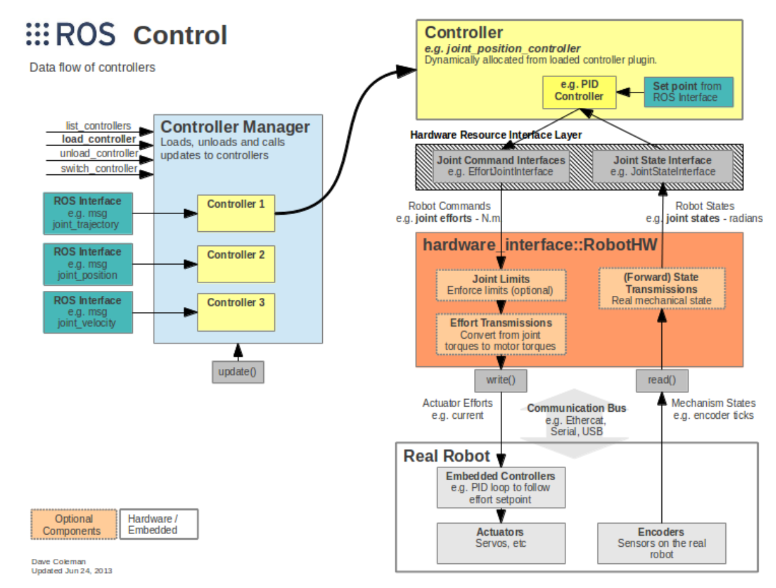
\includegraphics[width=\textwidth]{ros_control.png}\\
In the \textit{RACECAR project} we have six \textit{effort\_controllers}\footnote{Relative configuration can be found at 
\path{/catkin_ws/src/mit_racecar/racecar_gazebo/racecar_control/config/racecar_control.yaml}} form the ros\_control library,
they are PID controllers acting on the joint variables:
\begin{itemize}
    \item four, one for each wheel, of type \textit{joint\_velocity\_controller}, which receive a velocity setpoint
          and sends an effort output. They are pure proportional controllers with a gain of $1.0$ for the rear wheels, 
          and a gain of $0.5$ for the front tires;  
    \item two, one for each steering hinge, of type \textit{joint\_position\_controller}, which receive a position 
          input and sends an effort output. They are PD controllers with parameters $K_p = 1.0$ and $K_d = 0.5$;
\end{itemize}

The gazebo\_ros\_control plugin provides default ros\_control interfaces, and it also provides a pluginlib-based
interface to implement custom interactions between Gazebo and ros\_control for simulating more complex mechanisms.\\
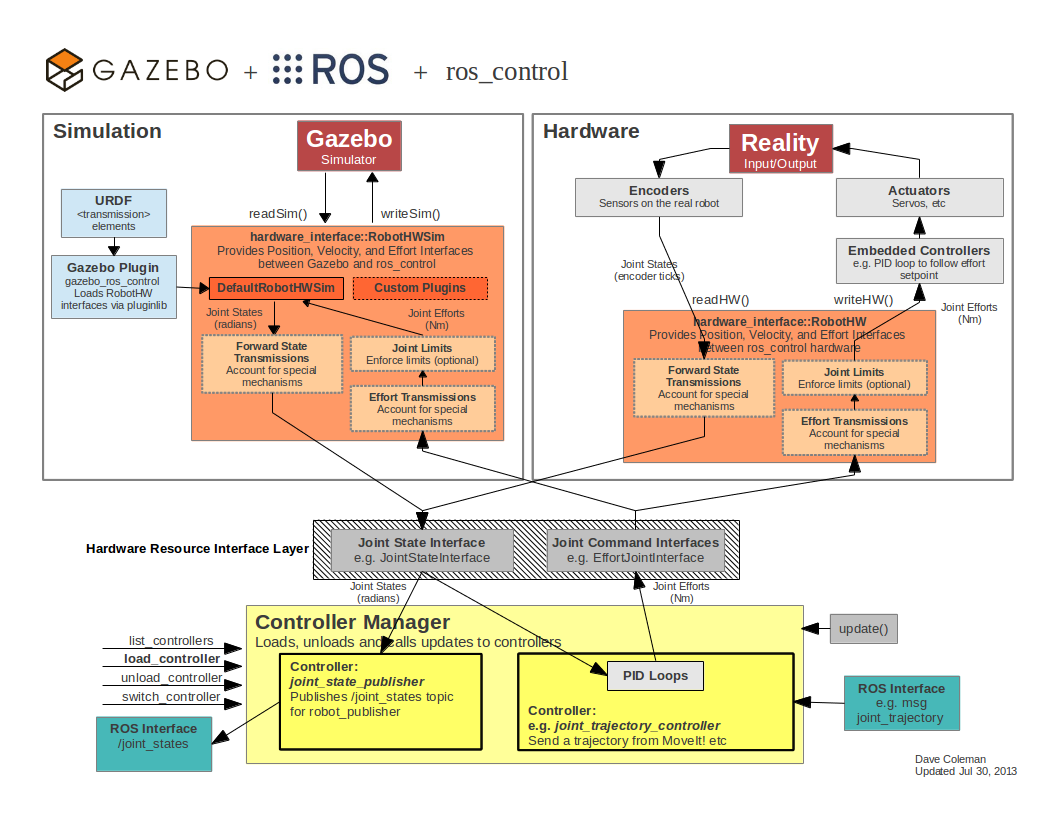
\includegraphics[width=\textwidth]{Gazebo_ros_transmission.png}\\
In order to use ros\_control within Gazebo, we need to enrich the URDF description adding <transmission> elements
in order to link actuators with joints. In our model, we have six transmissions: four to connect each wheel to a 
motor (with a mechanical reduction of $1$), and two connecting each steering hinge to a dedicated motor (also in
this case the mechanical reduction is $1$). \\
Finally, we add to the URDF file the gazebo\_ros\_control plugin by specifying the library filename ("libgazebo\_ros\_control.so")
and its parameters like a desired "robotNamespace".

\subsection{Laser plugin}
The Hokuyo laser plugin is specified in a \textit{Sensor} tag. It refers to the library 
\textit{libgazebo\_ros\_laser.so} which takes the role of controller of the laser 
(named \textit{gazebo\_ros\_hokuyo\_controller}).\\
This controller gathers range data from a simulated ray sensor, publishes range data using 
\textit{sensor\_msgs::LaserScan} messages on the ROS topic named \textit{/scan}.

\subsection{Camera plugin}
Similarly as the laser scan plugin the camera plugin is specified in a \textit{Sensor} tag. It refers
to the library \textit{libgazebo\_ros\_camera.so} which allows to control this sensor (the controller
is named \textit{camera\_controller}).\\
The camera publishes image messages on \textit{camera/zed/rgb/image\_rect\_color} ROS topic, while the
info messages are published on \textit{camera/zed/rgb/camera\_info}.\\
The coordinate frame where the image is published (tf tree) is \textit{camera\_link}.

\section{racecar\_gazebo code description}
In the previous sections we have illustrated how the model has been designed and its characteristics. In this
section we want to explain how the code is organized and the technical details of the implementation.\\
We will focus only on the \textit{racecar\_gazebo} package inside \textit{mit\_racecar}.

\subsection{racecar\_description}
The \textit{racecar\_description} package contains all specifications and files useful
to describe the car and the environments of the simulation.\\
In the \textit{urdf} folder there are four different XML files:
\begin{itemize}
    \item \textbf{macros.xacro}
    containing macros definitions for inertial parameters, geometries and transmissions
    for all the elements composing the car model. The usage of a xacro file allows to have a more readable 
    and organized code in the main URDF files.
    \item \textbf{materials.xacro} with the specification of the materials used in the car construction within
    Gazebo (in this case each material is simply determined by a RGB color that will be used for the visualization). 
    \item \textbf{racecar.xacro} which is the main description file. It contains all links, joints and transmissions
    composing the car model.\\
    It also includes all the other macro files and the Gazebo one.
    \item \textbf{racecar.gazebo} with friction parameters, plugin settings and all the additional 
    information needed to use URDF within a Gazebo simulation.
\end{itemize}
In the \textit{models} directory there are \textit{.config} and \textit{.sdf} files used to describe
the simulation environments. \\
The last folder is named \textit{meshes}, it contains \textit{.STL} and \textit{.dae} files which are the 3D models
of the car components used by Gazebo for the visual rendering.

\subsection{racecar\_gazebo}
In this package there are the files used to launch the Gazebo simulation.\\
In the \textit{worlds} folder we have several \textit{.worlds} files: they contain the description
of the available environments (worlds) in which the model can be simulated. \\
The second folder, named \textit{script}, contains the python implementation of \textit{gazebo\_odometry\_node}. 
This node is in charge of translating Gazebo status messages (coming from "/gazebo/link\_states" topic) to odometry data,
and then publishing it on "/vesc/odom" ROS topic at a \SI{20.0}{\hertz} rate. \\
The last folder is named \textit{launch} and contains one launch file for each world already implemented. \\
A launch file contains the list of ROS nodes to be spawned and their configuration; moreover, it can include
other \textit{.launch} files. Hence, we have a quick and tidy way to start the entire simulation. \\
In the package there are five \textit{.launch} files; the main one is \textit{racecar.launch}, while the others
only differ for the world in which the simulation will take place. \\
File \textit{racecar.launch} contains the following parts:  
\begin{itemize}
    \item world selection: it is specified the \textit{.world} file which describes the simulation environment (in this case
          an empty flat plane);
    \item robot description generation: the \textit{.xacro} file containing the description of the car model is converted 
          to URDF format and loaded into the parameter server;
    \item racecar spawning: \textit{racecar\_spawn} node, from \textit{gazebo\_ros} package, reads the model URDF from 
          the parameter server and implements it in the simulation; 
    \item call to \textit{racecar\_control.launch}: which loads all the joints effort controllers and starts the 
          \textit{servo\_commands} node; 
    \item call to \textit{mux.launch}: which creates a multiplexer to the handle different commands, having different priorities,
          received by the car. 
    \item topic remapping: \textit{better\_odom} node, from \textit{topic\_tools} package, uses the "relay" functionality 
          to subscribe to \textit{/vesc/odom} and republish to \textit{/pf/pose/odom}. 
\end{itemize}

\subsection{racecar\_control}
This package contains the logic of the car controllers.\\
In the \textit{scripts} we have the implementation of two ROS nodes:
\begin{itemize}
    \item \textit{keyboard\_teleop}\\
    Which allows the user to manually control the car by sending commands using the keyboard: \textit{W} to go forward,
    \textit{S} to move in reverse, \textit{A} and \textit{D} for turning left and right respectively. 
    Pressing a different key will stop the car, and by using the combination \textit{CTRL-C} the node is terminated and
    the controller stopped.\\
    A message of type \textit{AckermannDriveStamped} containing speed, acceleration, jerk, steering\_angle 
    and steering\_angle\_velocity is then published on the \textit{/vesc/ackermann\_cmd\_mux/input/teleop} topic to
    be sent to the car command mutiplexer.
    \item \textit{servo\_commands}\\
    The main purpose of this node is to read the information published on the \textit{/racecar/ackermann\_cmd\_mux/output} 
    topic by the multiplexer, and forward it to the various link controllers. \\
    It publishes the desired speed, pre-multiplied by 10, to the four wheel velocity controller topics; while,
    to the two hinge position controllers, it is forwarded the steering angle setpoints.
\end{itemize}
The second folder is named \textit{config}, it contains only one file which is \textit{racecar\_control.yaml}.
 A YAML file loads node configuration parameters in the ROS parameter server, it contains the information 
 about type, joint name and PID (proportional-integral-derivative) gain of each controller to be implemented 
 using the ros\_control library.

The \textit{launch} directory contains three launch files regarding controller functionalities:
\begin{itemize}
    \item \textit{gazebo\_sim\_joy.launch}\\
    starts the simulation in the tunnel environment and calls \textit{teleop.launch} (see below);
    \item \textit{racecar\_control.launch}\\
    loads the joint controller configurations from \textit{racecar\_control.yaml} to parameter server:
    Then it instantiates a \textit{controller\_manager}: a node (implemented in ros\_control) capable of spawning, loading, 
    unloading and updating all the controllers specified in the configuration file (.yaml file).
    Finally, it starts the aforementioned servo\_commands node. \\
    In addition, this file includes also some remapping of the topics used by the robot state publisher 
    (robot\_state\_publisher node), the robot movements controller (servo\_commands node) and the odometry publisher;
    \item \textit{teleop.launch} \\
    starts the \textit{keyboard\_teleop} node to allow the user to manually control the model.
\end{itemize}